
\begin{frame}[fragile]
  \frametitle{Universal Machine}
  \only<1>{
    Linguagens de programação interpretadas/avaliadas apresentam uma ``máquina'' chamada \var{eval}.
  }
  \only<2>{\begin{figure}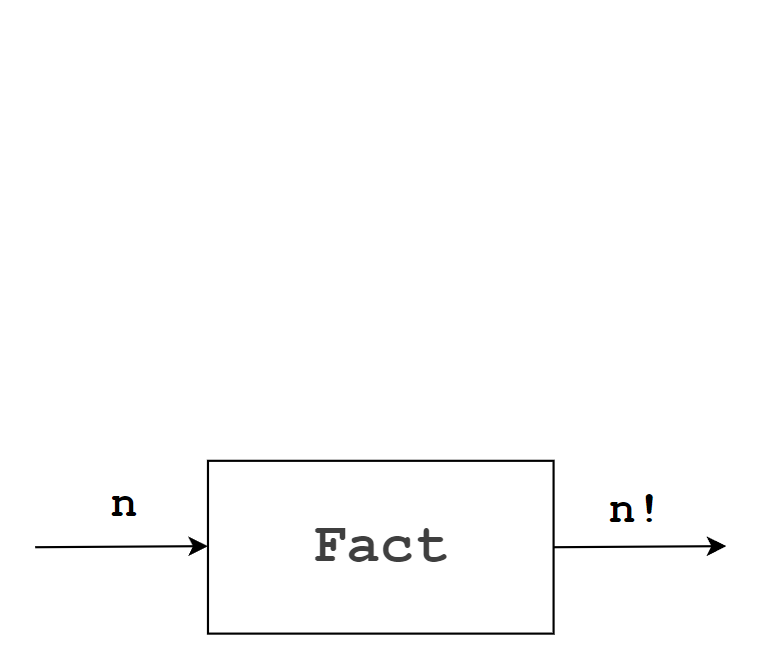
\includegraphics[width=0.5\textwidth]{fact3.png}\end{figure}}
  \only<3>{\begin{figure}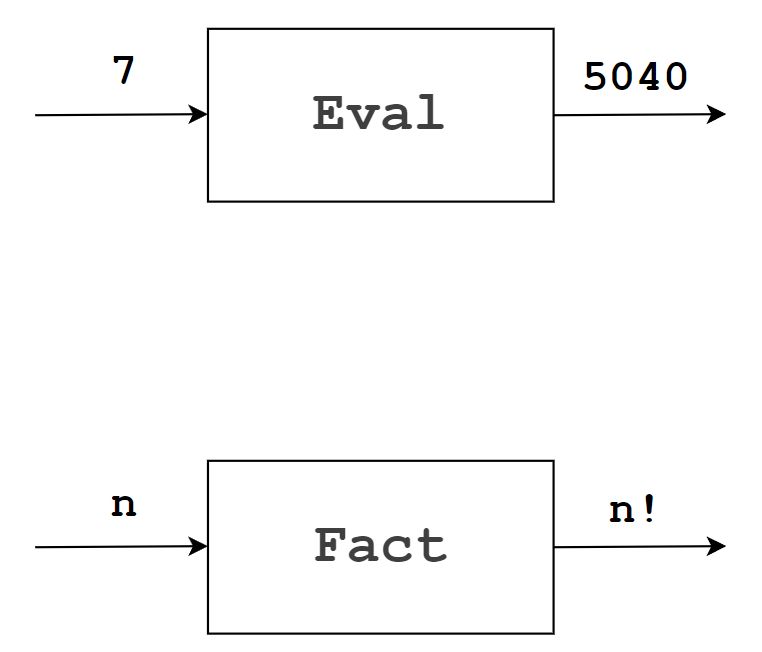
\includegraphics[width=0.5\textwidth]{fact2.png}\end{figure}}
  \only<4>{\begin{figure}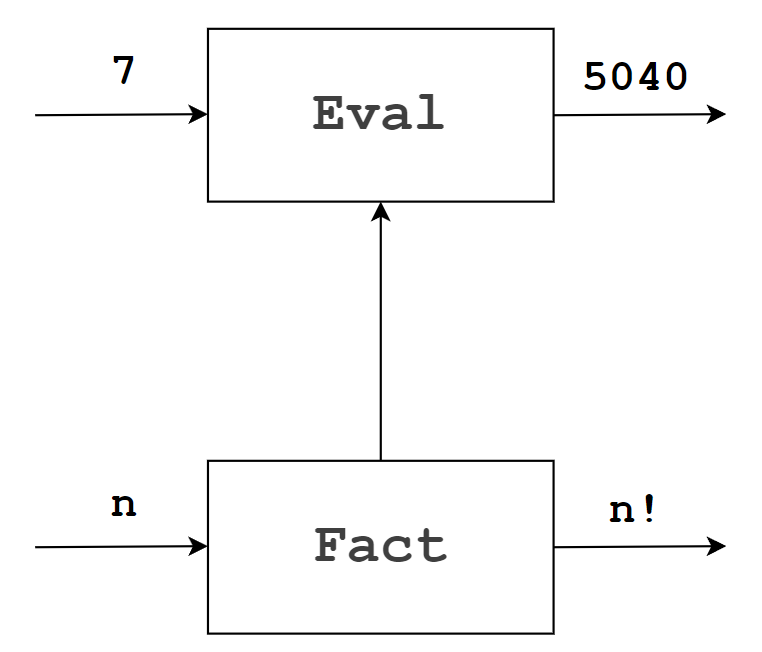
\includegraphics[width=0.5\textwidth]{fact1.png}\end{figure}}
  \only<5>{
    De maneira que essa construção, conhecida como \textit{Universal Machine}, seja um simulador (\textit{Describing Machine}) para a máquina \var{fact}, que, inclusive, é infinita.
  }
\end{frame}
